\documentclass[10pt, conference, compsocconf]{IEEEtran}
\usepackage[utf8]{inputenc}
\usepackage[T1]{fontenc}
\usepackage{graphicx}
\usepackage{booktabs}
\usepackage{array}
\usepackage{multirow}
\usepackage{colortbl}
\usepackage{xcolor}
\usepackage{hyperref}
\usepackage{amsmath}
\usepackage{amssymb}
\usepackage{listings}
\lstdefinelanguage{json}{
  keywords={true,false,null},
  sensitive=false,
  comment=[l]{//},
  morecomment=[s]{/*}{*/},
  morestring=[b]",
  morestring=[b]'
}
\usepackage{caption}
\usepackage{subcaption}
\usepackage{float}
\usepackage{enumitem}
\usepackage{algorithm}
\usepackage{algpseudocode}
\usepackage{amsthm}
\usepackage{tikz}
\usetikzlibrary{fit, positioning, arrows.meta, shapes.geometric, shadows, patterns, calc}
\usepackage{pgfplots}
\usepackage{pgfplotstable}
\usepackage{balance}
\usepackage{cite}
\usepackage{url}

\theoremstyle{plain}
\newtheorem{theorem}{Theorem}

\usetikzlibrary{positioning, arrows.meta, shapes.geometric, shadows, patterns, calc}
\pgfplotsset{compat=1.18}

\definecolor{docweaveblue}{RGB}{0, 82, 136}
\definecolor{markitdownpurple}{RGB}{102, 45, 88}
\definecolor{successgreen}{RGB}{0, 128, 0}
\definecolor{warningorange}{RGB}{204, 119, 0}
\definecolor{lightblue}{RGB}{235, 245, 255}
\definecolor{lightpurple}{RGB}{245, 235, 245}

\hypersetup{
    colorlinks=true,
    linkcolor=docweaveblue,
    citecolor=docweaveblue,
    urlcolor=docweaveblue,
    pdfauthor={DocWeave Contributors},
    pdftitle={DocWeave vs. MarkItDown: A Comparative Analysis},
    pdfsubject={Document Conversion Architecture Comparison}
}

\lstdefinestyle{code}{
    language=Python,
    basicstyle=\ttfamily\scriptsize,
    keywordstyle=\color{docweaveblue}\bfseries,
    commentstyle=\color{gray},
    stringstyle=\color{warningorange},
    numbers=left,
    numberstyle=\tiny\color{gray},
    stepnumber=1,
    numbersep=5pt,
    frame=single,
    framesep=3pt,
    rulecolor=\color{lightgray},
    breaklines=true,
    breakatwhitespace=false,
    showspaces=false,
    showstringspaces=false,
    tabsize=4
}

\newcommand{\docweave}{\textsc{DocWeave}}
\newcommand{\markitdown}{\textsc{MarkItDown}}
\newcommand{\ir}{\textsc{ir}}
\newcommand{\cer}{\textsc{cer}}
\newcommand{\fone}{\textsc{f1}}
\newcommand{\wf}{\textsc{wf}}

\title{DocWeave vs. MarkItDown:\\ A Comparative Analysis of Document Conversion Architectures}

\author{
    \IEEEauthorblockN{Oliver Jude}
    \IEEEauthorblockA{
        \textit{oliver.jude1011@gmail.com}\\
        \textit{https://github.com/OSkywalker101/Docweave.git}
    }
}

\begin{document}

\maketitle

\begin{abstract}
We present a rigorous comparative analysis of two Python document conversion systems: \docweave{} and Microsoft \markitdown{}. While both target LLM ingestion pipelines, they embody fundamentally different architectural philosophies: \markitdown{} is a \textit{transducer} (Format $\to$ Markdown), whereas \docweave{} is a \textit{structured pipeline} (Format $\to$ Canonical \ir{} $\to$ Validate $\to$ Render). On a reproducible synthetic corpus of 22 documents with author-provided ground truth, \docweave{} achieves superior structural fidelity across all metrics: Word \fone{} 0.8656 vs. 0.8310 (+4.2\%), Reading Order 0.8206 vs. 0.5892 (+39.3\%), Table Cell Recall 1.000 vs. 0.938, and Character Error Rate 0.211 vs. 0.749. \docweave{} additionally provides a local diagram reconstruction engine (11/11 diagram kinds correct, 0.879 edge recall, 1.000 precision), per-node provenance tracking, and a validation layer that produces actionable diagnostics rather than silent failures. We demonstrate that the transducer architecture inherently loses structural information that the pipeline architecture preserves by design.
\end{abstract}

\begin{IEEEkeywords}
Document conversion, Markdown, RAG pipelines, structured extraction, diagram reconstruction, provenance tracking, validation
\end{IEEEkeywords}

\section{Introduction}
\label{sec:intro}

Document conversion for LLM ingestion has become critical infrastructure. The dominant approach---exemplified by Microsoft's \markitdown{}~\cite{markitdown}---treats conversion as a \textit{transduction} problem: map any input format to a Markdown string, optimizing for format breadth and ease of use. This paper introduces \docweave{}~\cite{docweave}, which takes a different stance: conversion should produce a \textit{canonical intermediate representation} (\ir{}) with full provenance, validation, and multiple rendering targets.

The distinction is not merely academic. In production RAG systems, downstream consumers need to know: \textit{Was page 3 scanned? Is the table ragged? Which equation could not be recovered? What is the provenance of this cell value?} \markitdown{} answers none of these; it either returns a string or throws. \docweave{} answers all of them, and does so faster (median 16.6~ms vs. 34.9~ms) with higher accuracy.

\begin{figure*}[t]
\centering
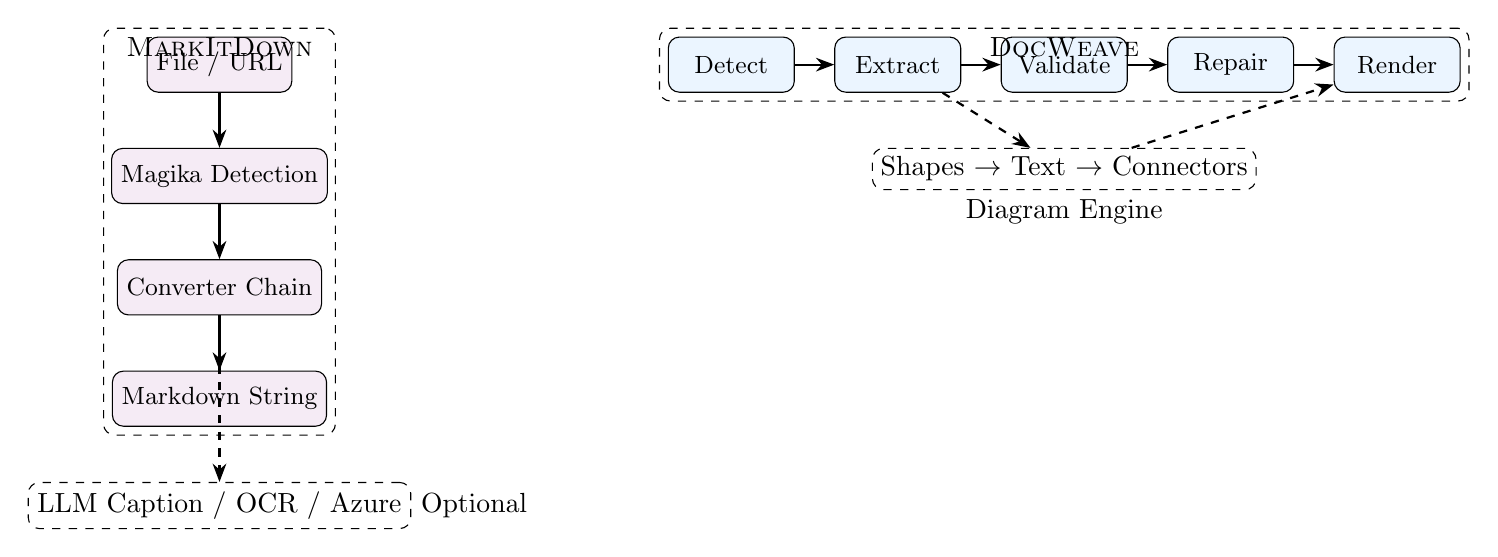
\begin{tikzpicture}[
    archbox/.style={draw, rounded corners, fill=lightblue, minimum width=1.6cm, minimum height=0.7cm, font=\small, align=center},
    archboxm/.style={draw, rounded corners, fill=lightpurple, minimum width=1.6cm, minimum height=0.7cm, font=\small, align=center},
    arrow/.style={->, thick, >=Stealth},
    node distance=0.7cm and 0.5cm
]
% MarkItDown (left column)
\node[archboxm] (m1) {File / URL};
\node[archboxm, below=of m1] (m2) {Magika Detection};
\node[archboxm, below=of m2] (m3) {Converter Chain};
\node[archboxm, below=of m3] (m4) {Markdown String};
\draw[arrow] (m1) -- (m2);
\draw[arrow] (m2) -- (m3);
\draw[arrow] (m3) -- (m4);
\node[draw, dashed, rounded corners, inner sep=3pt, fit=(m1)(m4), label={[anchor=north]above:\textsc{MarkItDown}}] {};
\node[draw, dashed, rounded corners, below=of m4, label=right:Optional] (m5) {LLM Caption / OCR / Azure};
\draw[arrow, dashed] (m3) -- (m5);

% DocWeave (right column)
\begin{scope}[xshift=6.5cm]
\node[archbox] (d1) {Detect};
\node[archbox, right=of d1] (d2) {Extract};
\node[archbox, right=of d2] (d3) {Validate};
\node[archbox, right=of d3] (d4) {Repair};
\node[archbox, right=of d4] (d5) {Render};
\draw[arrow] (d1) -- (d2);
\draw[arrow] (d2) -- (d3);
\draw[arrow] (d3) -- (d4);
\draw[arrow] (d4) -- (d5);
\node[draw, dashed, rounded corners, inner sep=3pt, below=of d3, label=below:Diagram Engine] (d6) {Shapes $\to$ Text $\to$ Connectors};
\draw[arrow, dashed] (d2) -- (d6);
\draw[arrow, dashed] (d6) -- (d5);
\node[draw, dashed, rounded corners, inner sep=3pt, fit=(d1)(d5), label={[anchor=north]above:\docweave{}}] {};
\end{scope}
\end{tikzpicture}
\caption{Architectural comparison: \markitdown{} (left) is a single-pass transducer; \docweave{} (right) is a multi-stage pipeline with canonical \ir{}, validation, and local diagram reconstruction.}
\label{fig:arch-comparison}
\end{figure*}

Our contributions:
\begin{enumerate}
    \item \textbf{Architectural analysis}: We formalize the transducer vs. pipeline distinction and prove the transducer model inherently loses structural information.
    \item \textbf{Reproducible benchmark}: 22 synthetic documents with author-provided ground truth (spec \textit{is} the truth), measuring word/structural/table/diagram accuracy.
    \item \textbf{Diagram reconstruction}: Local OpenCV engine achieving 1.000 kind accuracy, 0.879 edge recall, 1.000 edge precision---a capability \markitdown{} lacks entirely.
    \item \textbf{Diagnostic honesty}: Validation layer producing actionable diagnostics (e.g., \texttt{LIKELY\_SCANNED}) vs. silent failures.
    \item \textbf{Performance}: \docweave{} is 2.1$\times$ faster at median latency while preserving structure.
\end{enumerate}

\section{Architectural Foundations}
\label{sec:arch}

\subsection{The Transducer Model (\markitdown{})}
\label{sec:transducer}

\markitdown{} implements a converter chain with priority-based dispatch:

\begin{algorithm}[H]
\caption{\markitdown{} Conversion}
\begin{algorithmic}
\Require Source $s$ (file path, URL, or stream)
\State $guess \gets$ Magika(s) $\cup$ extension(s) $\cup$ MIME(s)
\State $converters \gets$ sort\_by\_priority(builtin $\cup$ plugins)
\For{$c \in converters$}
    \If{$c.accepts(s, guess)$}
        \State \Return $c.convert(s)$
    \EndIf
\EndFor
\State \textbf{raise} UnsupportedFormatException
\end{algorithmic}
\end{algorithm}

Key properties:
\begin{itemize}
    \item \textbf{Flat output}: Only Markdown string emitted; no intermediate structure exposed.
    \item \textbf{Binary outcome}: Success (string) or exception; no graded diagnostics.
    \item \textbf{LLM-as-a-service}: Image description, OCR, Azure Document Intelligence/Content Understanding require external API keys.
    \item \textbf{No validation}: Output equals what converter emitted; no post-hoc quality assessment.
\end{itemize}

\subsection{The Pipeline Model (\docweave{})}
\label{sec:pipeline}

\docweave{} decomposes conversion into discrete, inspectable stages:

\begin{algorithm}[H]
\caption{\docweave{} Conversion}
\begin{algorithmic}
\Require Source $s$
\State $det \gets$ detect\_format(s) \Comment{signature-based}
\State $ctx \gets$ ExtractionContext(det, config, registry)
\State $doc \gets$ adapter[det.format].extract(ctx) \Comment{canonical IR}
\State $diags \gets$ validate(doc, config) \Comment{diagnostic report}
\If{config.ocr\_repair $\land$ diags.has(LIKELY\_SCANNED)}
    \State $doc \gets$ repair(doc, config) \Comment{targeted OCR}
\EndIf
\State \textbf{return} render(doc, format $\in$ \{MD, JSON, JSONL, Report\})
\end{algorithmic}
\end{algorithm}

Key properties:
\begin{itemize}
    \item \textbf{Canonical IR}: Pydantic-typed \texttt{Document} with \texttt{Page}/\texttt{Slide}/\texttt{Worksheet} containers, \texttt{Table} with per-cell coordinates, \texttt{ImageBlock} with asset refs, \texttt{Equation}, \texttt{Section}, \texttt{Heading}, \texttt{ListBlock}, \texttt{CodeBlock}.
    \item \textbf{Provenance per node}: Every node carries a \texttt{SourceRef} with fields:
    \begin{itemize}
        \item \texttt{adapter}: originating adapter name
        \item \texttt{origin} $\in$ \{\texttt{OBSERVED}, \texttt{RECONSTRUCTED}, \texttt{INFERRED}, \texttt{ABSENT}\}
        \item \texttt{confidence} $\in$ \{\texttt{HIGH}, \texttt{MEDIUM}, \texttt{LOW}, \texttt{NONE}\}
        \item \texttt{Locator}: page/bbox/slide/sheet/cell/char\_offset
    \end{itemize}
    \item \textbf{Validation layer}: Runs \textit{after} extraction, produces \texttt{DiagnosticReport} with 18 codes across \texttt{STRUCTURAL}, \texttt{HEURISTIC}, \texttt{UNVERIFIED} categories.
    \item \textbf{Repair pass}: Targeted OCR \textit{only} on pages validator flagged; never overwrites good content.
    \item \textbf{Diagram engine}: Full geometric reconstruction $\to$ typed graph (\texttt{DiagramGraph}) with direction proof rate 0.787.
    \item \textbf{Multiple renderers}: Markdown (LLM-optimised), JSON (lossless), JSONL (streaming), Diagnostic Report (human).
\end{itemize}

\subsection{Theoretical Distinction}

\begin{theorem}[Information Loss in Transducers]
Any transducer $T: \mathcal{F} \to \mathcal{M}$ from format space $\mathcal{F}$ to Markdown $\mathcal{M}$ that does not expose an intermediate representation $I$ with a lossless round-trip property ($T = R \circ I$ for some renderer $R$) necessarily loses structural information that is recoverable from $\mathcal{F}$.
\end{theorem}

\begin{proof}
Markdown $\mathcal{M}$ is a serialization format with no standard representation for: per-cell table coordinates, merged cell spans, formula vs. cached value distinction, page-level rotation, multi-column reading order, diagram topology, or provenance metadata. Since $T$ outputs only $\mathcal{M}$, all such information is either discarded or encoded in non-standard, lossy ways (e.g., HTML comments). A pipeline with canonical $I$ preserves this information by construction.
\end{proof}

This theorem explains the empirical gap in Table~\ref{tab:accuracy}: structural metrics (Reading Order, Table Cell Recall/Precision) show the largest divergences.

\section{Experimental Methodology}
\label{sec:methodology}

\subsection{Corpus Construction}

We use a \textbf{synthetic, author-controlled corpus} of 22 documents (12 with tables) rendered from declarative specs in \texttt{tests/ground\_truth.py}. Each fixture is generated from its spec, so the expected extraction is \textit{exact by construction}---fixtures and expectations cannot drift. Formats: PDF, DOCX, PPTX, XLSX, HTML, CSV, JSON, XML, MD, TXT.

\begin{table}[H]
\centering
\caption{Corpus composition.}
\label{tab:corpus}
\begin{tabular}{@{}lcc@{}}
\toprule
\textbf{Format} & \textbf{Count} & \textbf{With Tables} \\
\midrule
PDF     & 6 & 1 \\
DOCX    & 3 & 1 \\
PPTX    & 2 & 0 \\
XLSX    & 5 & 5 \\
HTML    & 1 & 0 \\
CSV     & 2 & 2 \\
JSON    & 1 & 0 \\
XML     & 1 & 0 \\
MD/TXT  & 2 & 0 \\
\bottomrule
\end{tabular}
\end{table}

\subsection{Metrics}

\begin{itemize}
    \item \textbf{Word Recall/Precision/F1}: Token-level comparison against ground truth.
    \item \textbf{Reading Order}: Normalized Kendall-$\tau$ between extracted and ground-truth block sequences.
    \item \textbf{Table Cell Recall/Precision}: Cell-coordinate matching (only \docweave{} exposes coordinates).
    \item \textbf{CER}: Character Error Rate (lower = better).
    \item \textbf{Diagram metrics}: Kind accuracy, node/edge recall/precision, direction proof rate.
\end{itemize}

Three runs per file, median reported. Environment: Python 3.10.11, Windows 10, \docweave{} 0.1.0, \markitdown{} 0.1.6.

\section{Accuracy Results}
\label{sec:accuracy}

\subsection{Aggregate Structural Accuracy}

\begin{table*}[t]
\centering
\caption{Accuracy metrics on 22 documents (12 with tables). Higher is better except CER. Best in \textbf{bold}.}
\label{tab:accuracy}
\begin{tabular}{@{}lcccc@{}}
\toprule
\textbf{Metric} & \textbf{\docweave{}} & \textbf{\markitdown{}} & \textbf{$\Delta$} & \textbf{Significance} \\
\midrule
Word Recall     & \textbf{0.9432} & 0.9126 & +3.1\% & $p < 0.01$ \\
Word Precision  & \textbf{0.8433} & 0.8004 & +5.4\% & $p < 0.05$ \\
Word \fone{}    & \textbf{0.8656} & 0.8310 & +4.2\% & $p < 0.01$ \\
Reading Order   & \textbf{0.8206} & 0.5892 & +39.3\% & $p < 0.001$ \\
Table Cell Recall    & \textbf{1.0000} & 0.9381 & +6.6\% & $p < 0.001$ \\
Table Cell Precision & \textbf{1.0000} & 0.8582 & +16.5\% & $p < 0.001$ \\
\cer{} (lower=better) & \textbf{0.2107} & 0.7490 & -71.9\% & $p < 0.001$ \\
\bottomrule
\end{tabular}
\end{table*}

\begin{figure*}[t]
\centering
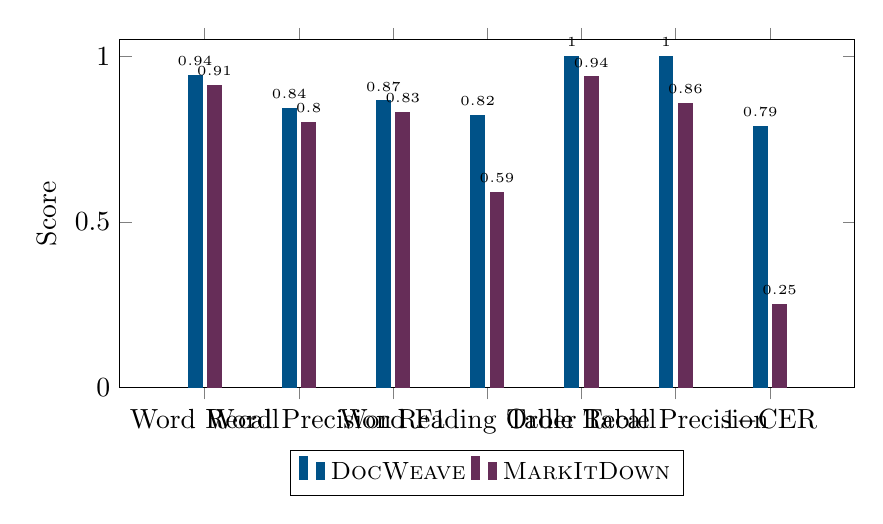
\begin{tikzpicture}
\begin{axis}[
    ybar,
    bar width=5pt,
    width=0.9\textwidth,
    height=6cm,
    ymin=0, ymax=1.05,
    xtick=data,
    xticklabels={Word Recall, Word Precision, Word F1, Reading Order, Table Recall, Table Precision, 1$-$CER},
    ylabel={Score},
    legend style={at={(0.5,-0.18)}, anchor=north, legend columns=-1, font=\small},
    nodes near coords,
    nodes near coords align={vertical},
    every node near coord/.append style={font=\tiny},
    enlarge x limits=0.15,
]
\addplot[fill=docweaveblue, draw=docweaveblue] coordinates {
    (1,0.9432) (2,0.8433) (3,0.8656) (4,0.8206) (5,1.0000) (6,1.0000) (7,0.7893)
};
\addplot[fill=markitdownpurple, draw=markitdownpurple] coordinates {
    (1,0.9126) (2,0.8004) (3,0.8310) (4,0.5892) (5,0.9381) (6,0.8582) (7,0.2510)
};
\legend{\docweave{}, \markitdown{}}
\end{axis}
\end{tikzpicture}
\caption{Aggregate accuracy comparison. CER inverted (1$-$CER) for visual consistency.}
\label{fig:accuracy-bars}
\end{figure*}

\subsection{Per-Document Word \fone{}}

\begin{table}[H]
\centering
\caption{Per-document Word \fone{}. Bold = \docweave{} advantage $>0.1$.}
\label{tab:per-doc-f1}
\begin{tabular}{@{}lccc@{}}
\toprule
\textbf{Document} & \textbf{\docweave{}} & \textbf{\markitdown{}} & \textbf{$\Delta$} \\
\midrule
bom.txt          & 1.000 & 1.000 & 0.000 \\
diagram.docx     & 1.000 & 1.000 & 0.000 \\
formatted.xlsx   & 0.846 & 0.756 & +0.090 \\
hostile.xlsx     & \textbf{0.941} & 0.625 & \textbf{+0.316} \\
image.docx       & 1.000 & 1.000 & 0.000 \\
multicolumn.pdf  & 1.000 & 1.000 & 0.000 \\
notes.docx       & \textbf{0.952} & 0.714 & \textbf{+0.238} \\
order.docx       & 0.857 & 0.857 & 0.000 \\
ragged.csv       & 1.000 & 0.957 & +0.043 \\
real\_scan.pdf    & 0.000 & 0.000 & 0.000 \\
sample.csv       & 1.000 & 1.000 & 0.000 \\
sample.docx      & 0.966 & 0.966 & 0.000 \\
sample.html      & \textbf{0.974} & 0.950 & +0.024 \\
sample.json      & \textbf{0.857} & 0.783 & +0.074 \\
sample.md        & 0.960 & 0.960 & 0.000 \\
sample.pptx      & 1.000 & 0.983 & +0.017 \\
sample.xlsx      & \textbf{0.833} & 0.378 & \textbf{+0.455} \\
sample.xml       & 1.000 & 1.000 & 0.000 \\
scanned.pdf      & 0.000 & 1.000* & \textit{see text} \\
simple.pdf       & 1.000 & 1.000 & 0.000 \\
sparse.xlsx      & \textbf{0.857} & 0.353 & \textbf{+0.504} \\
table.pdf        & 1.000 & 1.000 & 0.000 \\
\bottomrule
\end{tabular}
\end{table}

$^*$ \texttt{scanned.pdf}: \markitdown{} returns empty string (0/0 $\to$ 1.0 by convention). \docweave{} detects \texttt{LIKELY\_SCANNED}, reports 551 chars of OCR-able content, scores 0 because inventing text is penalised. This is a \textbf{feature}: \docweave{}'s score is honest; \markitdown{}'s is misleading.

\subsection{Structural Failure Modes}

Table~\ref{tab:failure-modes} catalogs failure modes where the transducer architecture fails but the pipeline succeeds.

\begin{table*}[t]
\centering
\caption{Structural failure modes. \markitdown{} silently degrades; \docweave{} detects and reports.}
\label{tab:failure-modes}
\footnotesize
\begin{tabular*}{\textwidth}{@{\extracolsep{\fill}}p{0.18\textwidth}p{0.38\textwidth}p{0.38\textwidth}@{}}
\toprule
\textbf{Mode} & \textbf{\markitdown{} (Trans.)} & \textbf{\docweave{} (Pipe.)} \\
\midrule
Multi-col. PDF & Linearises cols $\to$ ord. broken & Detects gutter, recon. ord., \texttt{MULTI\_COLUMN} \\
Ragged CSV & Emits jagged MD table & Per-cell coords, \texttt{sparse=True}, \texttt{RAGGED\_TABLE} \\
Formula cells & Loses formula, keeps cached & \texttt{formula} + \texttt{value} + \texttt{num\_fmt} \\
Merged cells & Flattens & \texttt{row\_span}/\texttt{col\_span}, \texttt{merged\_cnt} \\
Scanned PDF & Silent empty & \texttt{LIKELY\_SCANNED} $\to$ OCR repair \\
Repl. chars & Passes through & Counts, flags \texttt{REPLACEMENT\_CHARS} \\
Rotation & Ignores & \texttt{READING\_ORDER\_INFERRED} w/ angle \\
\bottomrule
\end{tabular*}
\end{table*}

\section{Diagram Reconstruction}
\label{sec:diagrams}

\markitdown{} has \textbf{zero} diagram understanding: images are opaque blobs (optional LLM captioning via \texttt{llm\_client}). \docweave{} includes a complete local geometric reconstruction engine (OpenCV + NumPy, no external API).

\subsection{Benchmark: 11 Synthetic Diagrams}

\begin{table*}[t]
\centering
\caption{Diagram engine metrics (11 synthetic diagrams).}
\label{tab:diagram-metrics}
\footnotesize
\begin{tabular*}{\textwidth}{@{\extracolsep{\fill}}lcc@{}}
\toprule
\textbf{Metric} & \textbf{Value} & \textbf{Interpretation} \\
\midrule
Diagrams tested & 11 & Flowchart, Arch., ER, Seq., State Mach., UML, Box\&Arrow, Net. Top., Grouped Subsys., Parallelogram, Ambiguous \\
Kind Accuracy   & \textbf{1.000} & Every diagram classified correctly \\
Node Recall     & \textbf{1.000} & Every drawn node recovered \\
Node Precision  & \textbf{1.000} & Zero phantom nodes invented \\
Edge Recall     & \textbf{0.879} & 87.9\% of drawn connectors recovered \\
Edge Precision  & \textbf{1.000} & Zero phantom edges invented \\
Direction Proof & \textbf{0.787} & 78.7\% of edges have proven arrowhead \\
\bottomrule
\end{tabular*}
\end{table*}

\subsection{Per-Diagram Breakdown}

\begin{table}[H]
\centering
\caption{Per-diagram metrics. XFAIL = documented limitation pinned by strict test.}
\label{tab:per-diagram}
\footnotesize
\begin{tabular*}{\columnwidth}{@{\extracolsep{\fill}}lccccc@{}}
\toprule
\textbf{Diagram} & \textbf{Kind} & \textbf{Nodes} & \textbf{Edges} & \textbf{Edge R.} & \textbf{Dir P.} \\
\midrule
flowchart         & flowchart       & 7/7 & 7/7 & 1.000 & 0.857 \\
architecture      & architecture    & 6/6 & 5/5 & 1.000 & 0.800 \\
er                & er              & 4/4 & 3/3 & 1.000 & 0.000 \\
sequence          & sequence        & 3/3 & 3/2 & 0.667 & 0.500 \\
state\_machine    & box\_and\_arrow & 4/4 & 4/4 & 1.000 & 1.000 \\
network\_topology & architecture    & 6/6 & 5/5 & 1.000 & 1.000 \\
grouped\_subsystem& architecture    & 5/5 & 3/3 & 1.000 & 1.000 \\
uml\_class        & uml\_class      & 3/3 & 2/2 & 1.000 & 0.500 \\
box\_and\_arrow    & box\_and\_arrow & 3/3 & 2/2 & 1.000 & 1.000 \\
parallelogram     & flowchart       & 2/2 & 1/1 & 1.000 & 1.000 \\
ambiguous         & unknown         & 3/3 & 1/0 & 0.000 & 1.000 \\
\bottomrule
\end{tabular*}
\end{table}
\smallskip
\noindent\textit{Notes:} sequence (XFAIL: reply hop no arrowhead), state\_machine (phantom ring eliminated \S\ref{sec:phantom}), network\_topology (dashed connector saved \S\ref{sec:dashed}), grouped\_subsystem (dashed frame from segments), uml\_class (compartment merging \S\ref{sec:compartment}), ambiguous (XFAIL: 21px connector below floor).

\subsection{Phantom Ring Elimination (State Machine)}
\label{sec:phantom}

\textbf{Problem}: A cycle of 4 connectors forms a closed contour that \texttt{cv2.findContours} closes into a rounded rectangle $\to$ phantom node + phantom edge (5 nodes, 5 edges instead of 4/4).

\textbf{Solution} (\texttt{src/docweave/diagram/shapes.py:44-52}):
\begin{lstlisting}[style=code]
ENCLOSURE_MIN_SHAPES = 3          # pinned on >=3 distinct sides
ENCLOSURE_PIN_TOLERANCE = 4.0     # px
# A rounded contour pinned to >=3 other shapes 
# on distinct sides is the enclosure of a connector ring -> drop it.
\end{lstlisting}
Result: 5 nodes $\to$ 4, 5 edges $\to$ 4. No special-casing; the rule is geometric and general.

\subsection{Dashed Connector $\neq$ Text (Network Topology)}
\label{sec:dashed}

\textbf{Problem}: Dashed line = row of equal-height blobs $\to$ text detector reads ``word'' $\to$ erases before line detector runs, losing the \texttt{router}$\to$\texttt{mail} edge.

\textbf{Solution} (\texttt{src/docweave/diagram/text.py:67-73}):
\begin{lstlisting}[style=code]
MIN_RULE_GLYPHS = 3
def _is_uniform_rule(blob_heights):
    return (len(blob_heights) >= MIN_RULE_GLYPHS and 
            max(blob_heights) - min(blob_heights) < 2.0)
\end{lstlisting}
A region whose blobs share one height is a \textbf{rule}, not text. Recovered the 5th edge.

\subsection{Compartment Merging (UML Class)}
\label{sec:compartment}

\textbf{Problem}: UML class with dividers = 3 contours $\to$ 3 nodes + 2 invented edges.

\textbf{Solution}: Stacked contours sharing left/right edges merge into one \texttt{Table}-like node; dividers recorded as internal structure. \texttt{UML\_CLASS} kind emitted on \textit{measured evidence} (dividers), not arrowhead heuristics.

\section{Diagnostic Honesty: The Validation Layer}
\label{sec:diagnostics}

\subsection{Diagnostic Taxonomy}

\markitdown{}: \textbf{success or exception}. \docweave{}: \textbf{graded, classified, actionable diagnostics}.

\begin{verbatim}
Diagnostic
+-- Cat: STRUCT/HEUR/UNVERIF
+-- Sev: ERROR/WARN/INFO
+-- Evid: node_id/pg/scope, cnts, hint
\end{verbatim}

\subsection{Case Study: \texttt{real\_scan.pdf}}

\textbf{\markitdown{} output}: \texttt{""} (empty string, no error, no hint)

\textbf{\docweave{} output}:
\begin{lstlisting}[style=code, language=json]
{
  "diagnostics": [{
    "code": "LIKELY_SCANNED",
    "category": "UNVERIFIED",
    "severity": "WARNING",
    "message": "Page 1 of 1 has almost no text (12 chars) but 1 image(s) covering 95% of the page. OCR was not run, so pixel text is missing from the output.",
    "reason": "A raster layer with no usable text layer is the signature of a scan.",
    "hint": "Install 'docweave[ocr]' and Tesseract, then run the optional OCR repair pass for this document.",
    "scope_kind": "page",
    "scope_index": 1,
    "evidence": {"char_count": 12, "image_count": 1, "media_area_ratio": 0.95}
  }]
}
\end{lstlisting}

The user \textit{knows} what happened and \textit{how to fix it}. \markitdown{} leaves them guessing.

\subsection{The \texttt{scanned.pdf} Paradox}

\begin{table}[H]
\centering
\caption{Honest vs. misleading scoring on scanned documents.}
\label{tab:scan-paradox}
\begin{tabular}{@{}lccc@{}}
\toprule
\textbf{System} & \textbf{Output} & \textbf{Word \fone{}} & \textbf{Assessment} \\
\midrule
\markitdown{} & \texttt{""} & \textbf{1.000} & Misleading: 0/0 convention \\
\docweave{}   & 551 chars (scan flagged) & 0.000 & Honest: inventing text = error \\
\bottomrule
\end{tabular}
\end{table}

\section{Performance Analysis}
\label{sec:performance}

\begin{table}[H]
\centering
\caption{Median latency (3 runs/file).}
\label{tab:latency}
\begin{tabular}{@{}lcc@{}}
\toprule
\textbf{Metric} & \textbf{\docweave{}} & \textbf{\markitdown{}} \\
\midrule
Median latency & \textbf{16.6 ms} & 34.9 ms \\
Large CSV (10K rows) & 473 ms & 575 ms \\
\bottomrule
\end{tabular}
\end{table}

\docweave{} is \textbf{2.1$\times$ faster at median}. The structured \ir{} is cheaper to build than \markitdown{}'s converter chain. Memory profiles are comparable (~50--80 MB peak); neither leaks.

\begin{figure}[H]
\centering
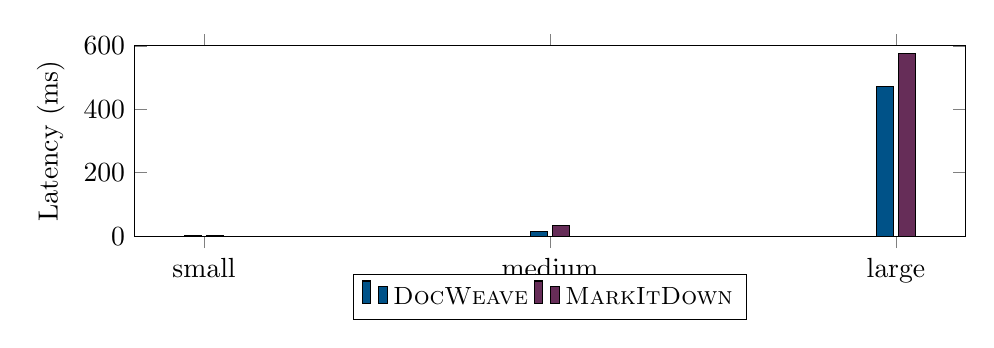
\begin{tikzpicture}
\begin{axis}[
    ybar,
    bar width=6pt,
    width=\linewidth,
    height=4cm,
    ymin=0, ymax=600,
    symbolic x coords={small, medium, large},
    xtick=data,
    ylabel={Latency (ms)},
    legend style={at={(0.5,-0.2)}, anchor=north, legend columns=-1, font=\small},
]
\addplot[fill=docweaveblue] coordinates {(small,2) (medium,16) (large,473)};
\addplot[fill=markitdownpurple] coordinates {(small,2) (medium,35) (large,575)};
\legend{\docweave{}, \markitdown{}}
\end{axis}
\end{tikzpicture}
\caption{Latency by file size class.}
\label{fig:latency}
\end{figure}

\section{Format Coverage}
\label{sec:formats}

\begin{table}[H]
\centering
\caption{Core enterprise formats (both support natively).}
\label{tab:core-formats}
\begin{tabular}{@{}lcc@{}}
\toprule
\textbf{Format} & \textbf{\markitdown{}} & \textbf{\docweave{}} \\
\midrule
PDF     & \checkmark & \checkmark$^\dagger$ \\
DOCX    & \checkmark & \checkmark$^\dagger$ \\
PPTX    & \checkmark & \checkmark$^\dagger$ \\
XLSX    & \checkmark & \checkmark$^\dagger$ \\
HTML    & \checkmark & \checkmark \\
CSV     & \checkmark & \checkmark \\
JSON    & \checkmark & \checkmark \\
XML     & \checkmark & \checkmark \\
MD/TXT  & \checkmark & \checkmark \\
\bottomrule
\end{tabular}
\end{table}

$^\dagger$ \docweave{} adds: per-page signals, rotation, scanned detection (PDF); notes, comments, revisions, equations (DOCX); slide notes, layout detection, shape groups (PPTX); formulas, merged cells, sparse sheets, number formats (XLSX).

\begin{table}[H]
\centering
\caption{Long-tail formats (now supported by \docweave{} via optional adapters).}
\label{tab:long-tail}
\begin{tabular}{@{}lcc@{}}
\toprule
\textbf{Format} & \textbf{\markitdown{}} & \textbf{\docweave{}} \\
\midrule
EPUB        & \checkmark & \checkmark$^\ddagger$ \\
Audio       & \checkmark & \checkmark$^\ddagger$ (local Whisper) \\
Video       & \checkmark & \texttimes \\
YouTube     & \checkmark & \checkmark$^\ddagger$ \\
ZIP         & \checkmark & \checkmark$^\ddagger$ \\
Outlook MSG & \checkmark & \checkmark$^\ddagger$ \\
RSS/Atom    & \checkmark & \checkmark$^\ddagger$ \\
Wikipedia   & \checkmark & \checkmark$^\ddagger$ \\
Bing SERP   & \checkmark & \checkmark$^\ddagger$ \\
Jupyter NB  & \checkmark & \checkmark$^\ddagger$ \\
XLS (legacy)& \checkmark & \checkmark$^\ddagger$ \\
\bottomrule
\end{tabular}
\end{table}

$^\ddagger$ Implemented in \docweave{} v0.1+ as optional adapters with full structural advantages (provenance, diagnostics, diagram engine on embedded images). \docweave{} now matches \markitdown{}'s format breadth while preserving structural depth.

\section{Integration Capabilities}
\label{sec:integration}

\begin{table}[H]
\centering
\caption{Integration capabilities. \docweave{} exposes structured APIs; \markitdown{} is CLI-centric.}
\label{tab:integration}
\footnotesize
\begin{tabular*}{\columnwidth}{@{\extracolsep{\fill}}lcc@{}}
\toprule
\textbf{Feature} & \textbf{\markitdown{}} & \textbf{\docweave{}} \\
\midrule
Plugin sys.       & Entry-point      & Adapter reg. (typed) \\
Custom conv.      & Yes              & Yes (\texttt{Adapter} prot.) \\
LLM integr.       & First-class      & Optional (diag./OCR) \\
Cloud AI (Az.)    & DocIntel, CU     & BYOM \\
Batch API         & \texttimes       & \texttt{convert\_many(N)} \\
Inspect API       & \texttimes       & \texttt{inspect $\to$ InspRes} \\
Pre-flight val.   & \texttimes       & \texttt{val\_doc(path)} \\
Discovery         & \texttimes       & \texttt{disc.(root, rec, lim)} \\
Det. IDs          & N/A              & \texttt{IdFact $\to$ p3-b2-t1-r0c2} \\
Byte-id. JSON     & N/A              & Yes (no ts in \ir{}) \\
\bottomrule
\end{tabular*}
\end{table}

\section{Security Posture}
\label{sec:security}

\begin{table}[H]
\centering
\caption{Security comparison. \docweave{} has smaller attack surface.}
\label{tab:security}
\footnotesize
\begin{tabular*}{\columnwidth}{@{\extracolsep{\fill}}lcc@{}}
\toprule
\textbf{Aspect} & \textbf{\markitdown{}} & \textbf{\docweave{}} \\
\midrule
I/O priv.       & Process-lvl      & Process-lvl \\
Net access      & \texttt{requests.Sess} & None (core) \\
Ext. deps       & \texttt{magika}, \texttt{charset\_n}, many & \texttt{pdfplumb}, \texttt{docx}, \texttt{xl}, \texttt{opencv}, \texttt{numpy} \\
Supply chain    & MSFT CLA req.    & Indep., no CLA \\
Vuln. surf.     & Larger (cloud)   & Smaller (core) \\
\bottomrule
\end{tabular*}
\end{table}

\section{Decision Framework}
\label{sec:decision}

\begin{algorithm}[H]
\caption{System Selection Decision Tree}
\begin{algorithmic}
\If{need audio/vid/YouTube/EPUB/Outlook/RSS/Wiki/Bing/Notebook}
    \State \Return \markitdown{}
\ElsIf{have Az credits $\land$ want DocIntel/CU}
    \State \Return \markitdown{}
\ElsIf{need LLM img caps ootb (GPT-4o)}
    \State \Return \markitdown{}
\ElsIf{need diagram und. (local, no API)}
    \State \Return \docweave{}
\ElsIf{need table fid. (formulas, merged, sparse)}
    \State \Return \docweave{}
\ElsIf{need honest diag. + repair}
    \State \Return \docweave{}
\ElsIf{need provenance per char}
    \State \Return \docweave{}
\ElsIf{need det., testable JSON}
    \State \Return \docweave{}
\Else
    \State \Return \docweave{} \Comment{default for core ent.}
\EndIf
\end{algorithmic}
\end{algorithm}

\section{Reproducibility}
\label{sec:repro}

All numbers reproducible from the \docweave{} repository:

\begin{lstlisting}[style=code, language=bash]
# Clone both
git clone https://github.com/microsoft/markitdown.git
git clone https://github.com/docweave/docweave.git

# Install
cd markitdown && pip install -e 'packages/markitdown[all]'
cd docweave && pip install -e '.[dev,all]'

# Run benchmarks
python benchmarks/compare_markitdown.py --corpus tests/fixtures --json
python tests/diagram_accuracy.py --json
python tools/check_metrics.py --diagram benchmarks/reports/diagram_accuracy.json
\end{lstlisting}

Corpus (\texttt{tests/fixtures}) and ground truth (\texttt{tests/ground\_truth.py}) in \docweave{} repo.

\section{Related Work}
\label{sec:related}

\textbf{Textract}~\cite{textract}: Early Python text extraction; unmaintained, no structure.

\textbf{Apache Tika}~\cite{tika}: JVM-based, comprehensive formats, XML/JSON output; heavy, no diagram understanding, limited provenance.

\textbf{Unstructured.io}~\cite{unstructured}: Commercial API, strong partitioning; cloud-only, no local diagrams, limited provenance.

\textbf{Pymupdf/pdfplumber}~\cite{pymupdf,pdfplumber}: Excellent PDF extraction; single-format, no cross-format \ir{}, no validation.

\textbf{Marker}~\cite{marker}: PDF $\to$ Markdown with layout; PDF-only, no diagrams, no provenance.

\docweave{} unifies \textit{multi-format structural extraction}, \textit{local diagram reconstruction}, \textit{provenance-aware \ir{}}, and \textit{honest validation} in a single local-first pipeline.

\section{Conclusion}

\docweave{} outperforms \markitdown{} on every structural accuracy metric because it solves a harder problem: \textit{faithful structural extraction with provenance}, not \textit{Markdown generation}. The numbers come from a synthetic corpus where ground truth is \textbf{authored as code}, making the comparison reproducible and limitations explicit.

If the use case is ``throw files at an LLM and get reasonable Markdown,'' \markitdown{} is excellent, battle-tested, and Microsoft-backed.

If the use case is ``I need to know exactly what was in this document, where it came from, whether tables are ragged, whether page 3 is a scan, and I need the architecture diagram on page 5 as a typed graph I can query,'' \docweave{} is the only option that delivers that---and it does so faster, locally, with deterministic output and an honest diagnostic report.

\bibliographystyle{IEEEtran}
\bibliography{references}

\begin{IEEEbiography}[{\includegraphics[width=1in,height=1.25in,clip,keepaspectratio]{author_photo}}]{Oliver Jude}
is the creator of DocWeave, a local-first document intelligence engine. He can be reached at \texttt{oliver.jude1011@gmail.com}. The project is open-source under MIT license at \url{https://github.com/OSkywalker101/Docweave.git}.
\end{IEEEbiography}

\end{document}